\documentclass{standalone}
\usepackage{times}
\usepackage{mathtools}

\usepackage{tikz}
\usetikzlibrary{positioning,fit,shapes,calc,decorations.pathreplacing}
\usetikzlibrary{backgrounds}
\usetikzlibrary{arrows.meta}
\usetikzlibrary{shapes,snakes}

\definecolor{processblue}{cmyk}{1,1,1,0}
\definecolor{accent}{rgb}{0.6,0.6,0.6}
\definecolor{accent2}{rgb}{0.9,0.9,0.9}

\begin{document}
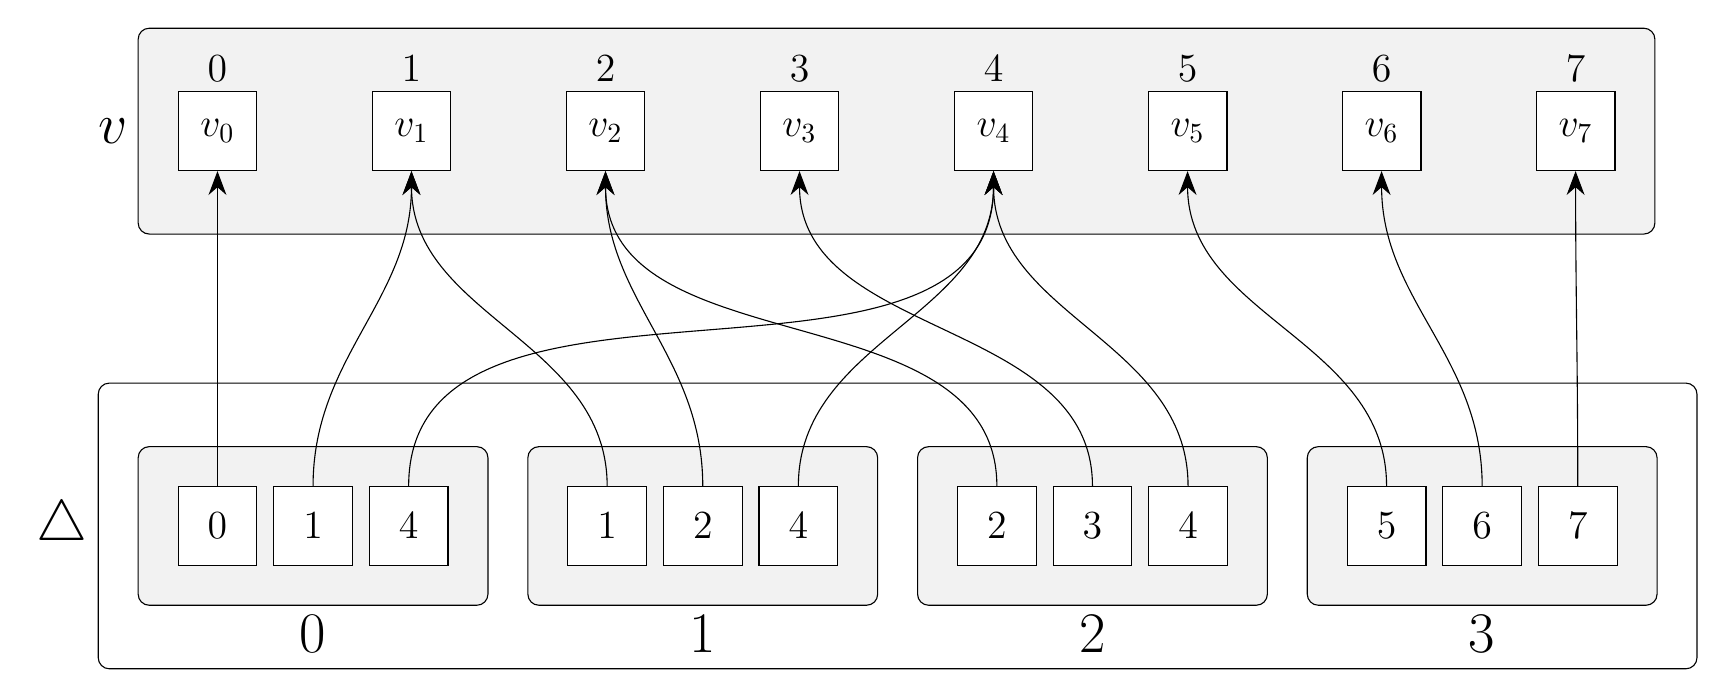
\begin{tikzpicture}[
  data/.style = {
    draw,
    rectangle,
    fill = white,
    minimum width = 1.0cm,
    minimum height = 1.0cm,
  },
  next/.style = {
    draw,
    circle,
    fill=black,
  },
  edge/.style = {
    draw,
    rectangle,
    rounded corners,
    minimum width = 0.5cm,
    minimum height = 0.5cm,
  },
  vedge/.style = {
    edge,
    top color = black!5,
    bottom color = black!5,
  },
  fedge/.style = {
    edge,
    top color = accent,
    bottom color = accent,
  },
  >={Stealth[scale=1.8]},
]

  % \clip (-3.5,-3.0) rectangle (18,2.5);

  \node[data,label={\Large $0$}] (v0) {\Large $v_0$};
  \node[data,label={\Large $1$}] (v1) [right=1.45cm of v0] {\Large $v_1$};
  \node[data,label={\Large $2$}] (v2) [right=1.45cm of v1] {\Large $v_2$};
  \node[data,label={\Large $3$}] (v3) [right=1.45cm of v2] {\Large $v_3$};
  \node[data,label={\Large $4$}] (v4) [right=1.45cm of v3] {\Large $v_4$};
  \node[data,label={\Large $5$}] (v5) [right=1.45cm of v4] {\Large $v_5$};
  \node[data,label={\Large $6$}] (v6) [right=1.45cm of v5] {\Large $v_6$};
  \node[data,label={\Large $7$}] (v7) [right=1.45cm of v6] {\Large $v_7$};

  \node[data] (f00) [below=4cm of v0] {\Large $0$};
  \node[data] (f01) [right=0.2cm of f00] {\Large $1$};
  \node[data] (f02) [right=0.2cm of f01] {\Large $4$};
  \begin{scope}[on background layer]
    \node[vedge,fit=(f00) (f02),inner sep=0.5cm,label={below: \huge $0$}] (f0) {};
  \end{scope}

  \node[data] (f10) [right=of f0] {\Large $1$};
  \node[data] (f11) [right=0.2cm of f10] {\Large $2$};
  \node[data] (f12) [right=0.2cm of f11] {\Large $4$};
  \begin{scope}[on background layer]
    \node[vedge,fit=(f10) (f12),inner sep=0.5cm,label={below: \huge $1$}] (f1) {};
  \end{scope}

  \node[data] (f20) [right=of f1] {\Large $2$};
  \node[data] (f21) [right=0.2cm of f20] {\Large $3$};
  \node[data] (f22) [right=0.2cm of f21] {\Large $4$};
  \begin{scope}[on background layer]
    \node[vedge,fit=(f20) (f22),inner sep=0.5cm,label={below: \huge $2$}] (f2) {};
  \end{scope}

  \node[data] (f30) [right=of f2] {\Large $5$};
  \node[data] (f31) [right=0.2cm of f30] {\Large $6$};
  \node[data] (f32) [right=0.2cm of f31] {\Large $7$};
  \begin{scope}[on background layer]
    \node[vedge,fit=(f30) (f32),inner sep=0.5cm,label={below: \huge $3$}] (f3) {};
  \end{scope}

  \begin{scope}[on background layer]
    \node[vedge,fit=(v0) (v7),label={left: \huge $v$},inner sep=0.5cm,inner ysep=0.8cm] (v) {};
    \node[edge,fit=(f0) (f3),label={left:\huge $\triangle$},inner sep=0.5cm,inner ysep=0.8cm] (f) {};
  \end{scope}

  \path[->] (f00) edge node {} (v0);
  \path[->] (f01) edge[out=90,in=-90] node {} (v1);
  \path[->] (f02) edge[out=90,in=-90] node {} (v4);

  \path[->] (f10) edge[out=90,in=-90] node {} (v1);
  \path[->] (f11) edge[out=90,in=-90] node {} (v2);
  \path[->] (f12) edge[out=90,in=-90] node {} (v4);

  \path[->] (f20) edge[out=90,in=-90] node {} (v2);
  \path[->] (f21) edge[out=90,in=-90] node {} (v3);
  \path[->] (f22) edge[out=90,in=-90] node {} (v4);

  \path[->] (f30) edge[out=90,in=-90] node {} (v5);
  \path[->] (f31) edge[out=90,in=-90] node {} (v6);
  \path[->] (f32) edge[out=90,in=-90] node {} (v7);

\end{tikzpicture}
\end{document}
